\chapter{Background}\label{sec:Background}
Reinforcement learning (RL) is a process that requires on one hand interactive parts and on the other algorithms that improve interactions. The following section \ref{reinforcement_learning} introduces the general concept of RL and its specifications. Afterwards, two popular learning algorithms for RL problems are presented: Proximal Policy Optimization (PPO) and the training approach of a deep Q-Network (DQN).

\section{Reinforcement Learning}\label{reinforcement_learning}
%https://lilianweng.github.io/lil-log/2018/02/19/a-long-peek-into-reinforcement-learning.html#key-concepts
\marginpar{rl components}
Sutton and Barto wrote in ``Reinforcement learning: An introduction'' \cite{suba18} that RL is based on two components that interact with each other: an environment and an agent, see Figure \ref{fig:rl_cycle}. Those interactions take part during a time period with discrete time steps $t\in\mathbb{N}_0$ until a goal is reached or the ending condition applies. Formally, the journey of the agent finding the goal state is described as the Markov Decision Process (MDP). Often, an agent can only see a small field of view, which turns an MDP to a partially observable MDP.
% and every decision on the way is part of a reinforcement learning method. 
When multiple agents act in the same environment the Markov decision process is called a stochastic game \cite{buba10}.
% Initially the agent gets a starting environment state $S_0$, and can processes it to choose and execute an action $A_0$. This concludes the first time step. The environment changes based on the action and transitions into the next state $S_{1}$. In return the the agent receives the new state with a reward $R_{1}$ rating the action $A_0$. Afterwards the agent proceeds to execute actions which leads to the displayed cycle of Figure \ref{fig:rl_cycle}.
\begin{figure}[hpbt]
    \centering
    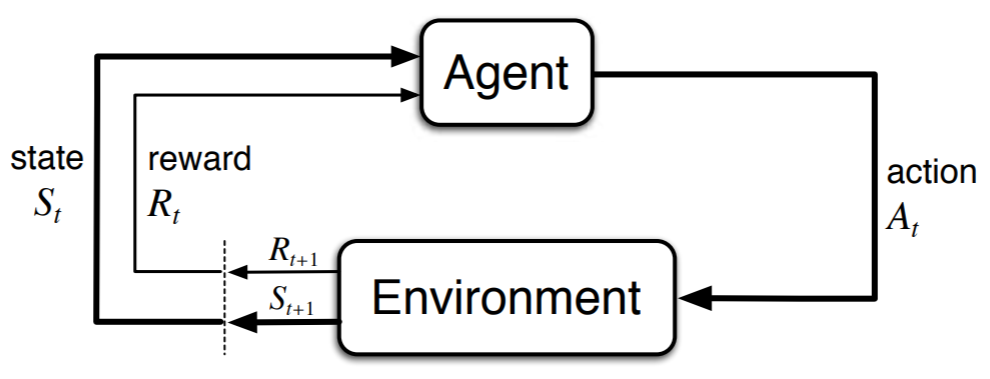
\includegraphics[width=0.6\textwidth]{pictures/RLInteractionSB}\\
    \caption[Reinforcement Learning Cycle]{The cycle of agent-environment interaction as
        shown in ``Reinforcement learning: An introduction'' \cite{suba18}}\label{fig:rl_cycle}
\end{figure}

\marginpar{sets and values}
One environment state $S_t$ is part of a set $S$ containing all possible states. During each point in time $t$ the agent can interact with the environment by executing an action $A_t$, which in turn changes the environment state. Since it is possible that not all actions are valid in each state the agents action selection is based on a restricted set $A_t\in A(S_t)$. In a multiagent environment, every agent chooses its action and adds it into a joint action set, which is executed collectively during $t$ \cite{buba10}.

The reward $R_t$ is element of a set of possible rewards $R$, which is a subset of real numbers $R \subset \mathbb{R}$. Therefore, the reward can potentially be negative or very low. Depending on the environment, that value can act as immediate feedback to the agents action. The general concept of RL, as defined by Sutton and Barto, is for agents to maximize rewards. Unlike machine learning approaches, the agent starts with no knowledge about good or bad actions and enhances the decision-making over time.

\marginpar{policy}
Sutton and Barto continue by defining the agents action selection with respect to the current state as a policy $\pi$. They explain further that a policy could be as simple as a lookup table, mapping states to actions, or it could contain a complicated search process for the best decision.
In most cases however, policies map action-state pairs to a selection probability, with all actions of a state adding up to 100\%.
During environment interactions agents receive rewards, which then can be used to update the policy accordingly. For a negative or low reward as an example, the probability of policy $\pi(a \mid s)$ decreases, reducing the chances of executing that same action in that specific state again.

\marginpar{value function}
While rewards only rate the immediate situation, a value function, i.e. the state-value function $V^\pi(s_t)$ for a policy $\pi$, can be used to estimate the long-term value of a state $s$ \cite{suba18}:
% \begin{equation}\label{eq:value_func}
%     V^\pi(s_t) = r_t + \gamma r_{t+1} + \gamma^2 r_{t+2} + \cdots = \sum^{\infty}_{i=0} \gamma^i r_{t+i}
% \end{equation}
\begin{equation}\label{eq:value_func}
    v_\pi(s) \doteq \mathbb{E}_\pi \left[ G_t \mid S_t = s \right] = \mathbb{E}_\pi \left[ \sum^{\infty}_{k=0} \gamma^k R_{t+k+1 \mid S_t = s}  \right]
\end{equation}
The result is the estimated discounted cumulative reward, an agent could get following that state and choosing actions based on the current policy. The discount factor is defined by Sutton and Barto as $0 \le \gamma < 1$ and provides a constant that reduces the importance of future rewards. A high $\gamma$ symbolizes a greater interest in rewards that are far away, whereas a discount of zero only takes the immediate reward into account. By setting $\gamma$ smaller than one it is ensured that the infinite sum results in a value.

Generally, states that offer immediate high rewards could end in a 
% The value function is of importance, due to states bringing high rewards could end in
low reward streak. In the opposite case, a low reward state could subsequently yield high rewards. Therefore, value functions are of great use to achieve the maximum reward.
% Other value functions can also take the executed
% action into account to reach the state from which the rewards are estimated.

\marginpar{exploration vs exploitation}
The last part to note about RL is that it entails the problem of balancing exploration and exploitation. On one hand, an agent has to explore the options given in order to learn and expand its knowledge. On the other hand, agents strive to maximize the reward, which can lead to greediness. An agent could start exploiting its knowledge too early,  choosing actions of which it knows to result in positive rewards. However, if an agent does not explore enough the best action sequence will stay hidden and the agents' knowledge will not improve.
%  In the opposite case, when an agent always explores without exploiting its knowledge, it is very likely that the reward will not be optimal. Finding the trade off between the two strategies is a common RL challenge.

\section{Proximal Policy Optimization}
\marginpar{intro}
In 2017 Schulman et al. introduced the concept of PPO in
the article ``Proximal Policy Optimization Algorithms'' \cite{scwo17}.
This section is solely based on that article in order to explain the Algorithm.
Policy optimization is the improvement of the action selection strategy $\pi$ based on the current state $s_{t}$. This is achieved by rotating two steps: 1. Sampling data from the policy and 2. Optimizing that data through several epochs.

\marginpar{TRPO}
The origin of PPO lies in a similar approach called Trust Region Policy Optimization (TRPO). TRPO strives to maximize the following function:
\begin{equation}\label{eq:TRPO}
    \underset{\theta}{maximize}\,\hat{\mathbb{E}}_{t} \left[ \frac{\pi_{\theta}(a_{t} \mid s_{t})}{\pi_{\theta_{old}}(a_{t} \mid s_{t})}
        \hat{A}_{t}-\beta \, KL[\pi_{\theta_{old}}(\cdot \mid s_{t}),\pi_{\theta}(\cdot \mid s_{t})] \right]
\end{equation}
The expectation $\hat{\mathbb{E}}_{t}$ indicates, that an  empirical average over a number $t$ of samples is used for estimation, and the algorithm alternates between sampling and executing these calculations.
 
\marginpar{TRPO advantage func}
The variable $\hat{A}_{t}$ describes an estimator of the advantage function. This function was defined in the paper ``Trust Region Policy Optimization'' \cite{scle15} with \\ $A_\pi(s,a) = Q_\pi(s,a)-V_\pi(s)$. The first part calculates the state-action value, estimating the upcoming rewards for an agent, starting at state s and initially selecting action a. Afterwards, the action selection is based on the current policy $\pi$. 

\marginpar{TRPO advantage func 2}
The second part contains the state value function $V_\pi(s)$, which works very similarly by starting at state s and using the policy. However, the difference is that the agent always chooses actions according to the policy. The advantage that is produced by the function $A_\pi(s,a)$ shows, whether a profit could be gained when deviating from the policy, by specifically choosing action a.

\marginpar{r(theta)}
The fraction $\frac{\pi_{\theta}(a_{t} \mid s_{t})}{\pi_{\theta_{old}}(a_{t} \mid s_{t})}$ in the Minuend of function \eqref{eq:TRPO} can be replaced by $r(\theta)$
%= \frac{\pi_{\theta}(a_{t} \mid s_{t})}{\pi_{\theta_{old}}(a_{t} \mid s_{t})}$
and represents the probability ratio of an action in the current policy in comparison to the old policy. Here,  $\theta$ represents a policy parameter. The result of $r(\theta)$ is greater than one, if an action is very probable in the current policy. Otherwise, the outcome lies between zero and one. Schulman et al. further extract the first part of function \eqref{eq:TRPO} as the surrogate objective:
\begin{equation}\label{eq:TRPO_surrogate}
    L^{CPI}(\theta) = \hat{\mathbb{E}}_{t} \left[ \frac{\pi_{\theta}(a_{t} \mid s_{t})}{\pi_{\theta_{old}}(a_{t} \mid s_{t})} \hat{A}_{t} \right]
    = \hat{\mathbb{E}}_{t} \left[ r(\theta)\hat{A}_{t} \right]
\end{equation}
However, maximized on its own without a penalty, this results in a large outcome and leads to drastic policy updates.

\marginpar{problem TRPO}
In order to stay in a trust region, as the name suggests, a penalty is subtracted from the surrogate function \eqref{eq:TRPO_surrogate}. The penalty is the Subtrahend of equation \eqref{eq:TRPO} and contains the fixed coefficient $\beta$. Regardless of the function details and outcome of $KL$, the coefficient $\beta$ is hard to choose, since different problems require different penalty degrees. Even during a TRPO run it could be necessary to adapt the coefficient, due to changes.

\marginpar{PPO}
Therefore Schulman et al. introduced
\begin{equation}\label{eq:PPO}
    L^{CLIP}(\theta) = \hat{\mathbb{E}}_{t} \left[ \min \left( \; r(\theta)\hat{A}_{t}, \quad clip(r(\theta), 1-\epsilon, 1+\epsilon)\hat{A}_{t} \; \right) \right]
\end{equation}
which is very similar to equation \eqref{eq:TRPO} but does not require coefficients. The first $\min$ entry contains $L^{CPI}$ \eqref{eq:TRPO_surrogate}. The second part contains a $clip$ function which narrows the space of policy mutation with the small hyperparameter $\epsilon$. After applying the clip function $r(\theta)$ lies between $[1-\epsilon,1+\epsilon]$. Calculating the minimum of the clipped and unclipped probability ratio produces the lower bound of the unclipped $r(\theta)$, preventing the policy to change drastically.

\marginpar{PPO Algo}
Finally, PPO is introduced with the following equation
\begin{equation}\label{eq:PPO_algo}
    L_{t}^{CLIP+VF+S}(\theta) = \hat{\mathbb{E}}_{t} \left[ L_{t}^{CLIP}(\theta) - c_{1}L_{t}^{VF}(\theta) + c_{2}S[\pi_{\theta}](s_{t}) \right]
\end{equation}
with $c_{1}$ and $c_{2}$ as coefficients. The authors point out that the loss function \\
$L_{t}^{VF} = (V_{\theta}(s_{t})-V_{t}^{targ})^2$ combines the policy surrogate and the value function error term and is necessary once a neural network shares parameters between policy and value function. Additionally, an entropy bonus $S$ is added to ensure exploration.

Furthermore, Schulman et al. point out that the policy is executed for $T$ time steps, with $T$ being a smaller value than the overall episode duration. Until now, the advantage function calculates values that run over an infinite loop, see the value function \eqref{eq:value_func} for example. Therefore, the advantage function needs to be adjusted as well. It is necessary that the future estimations do not exceed that time step limit. In this context the following advantage function is used:
\begin{equation}\label{eq:advantage_func}
    \hat{A_t} = \delta_t+(\gamma \lambda)\delta_{t+1}+ \cdots + (\gamma \lambda)^{T-t+1}\delta_{T-1}
\end{equation}
\begin{equation}\label{eq:advantage_func_delta}
    \textrm{where} \qquad \delta_t = r_t + \gamma V(s_{t+1}) - V(s_t)
\end{equation}

\marginpar{AC}
Schulman et al. also showed an example of the Algorithm using PPO with an actor-critic approach, see Fig. \ref{fig:ppo_algo_code}. According to Konda and Tsitsiklis \cite{kots03}, A critic is responsible to approximate the value function of the policy, and the actor in turn improves the policy based on the approximation results of the critic.

\marginpar{PPO pseudo}
Here, $N$ detonates actors collecting data in T time steps in each Iteration. Meanwhile, the critic computes the estimations of the advantage values. Afterwards, the policy is replaced with a new one, in which the function $L_{t}^{CLIP+VF+S}(\theta)$ \eqref{eq:PPO_algo} is optimized during K epochs. For the optimization process a small random batch of the previous time steps is used.
\begin{figure}[hpbt]
    \centering
    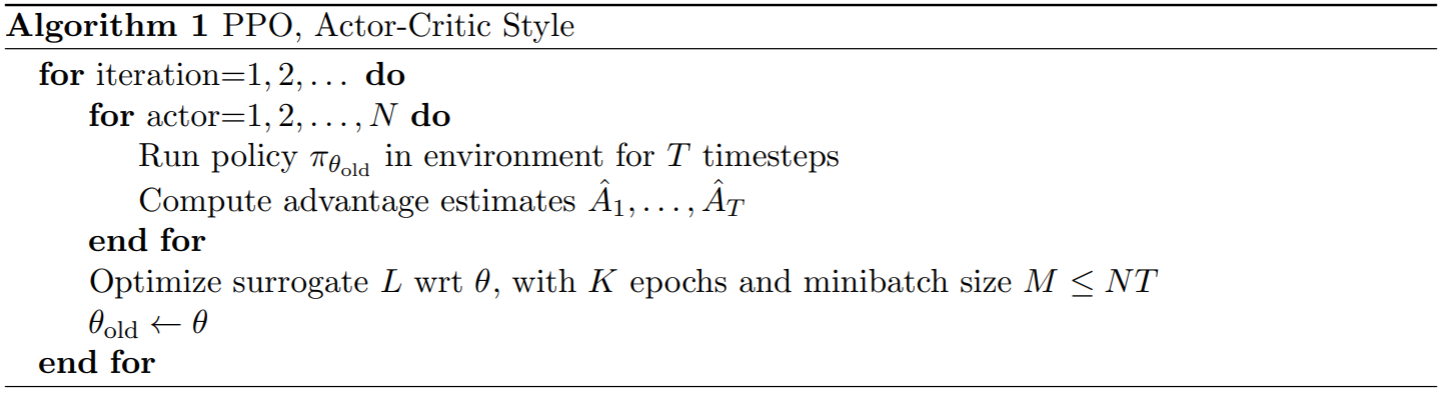
\includegraphics[width=1\textwidth]{pictures/ppo_algo_code.png}\\
    \caption[Exemplary Use Of PPO]{Exemplary use of PPO, as shown in ``Proximal Policy Optimization Algorithms'' \cite{scwo17}}\label{fig:ppo_algo_code}
\end{figure}

\section{Deep Q-Network}\label{dqn}
\marginpar{q value function}
Another learning approach often compared with PPO is the training of a deep Q-Network with Q-learning and experience replay. This algorithm relies on the action value function, that is formally defined as follows \cite{mnba16}:
\begin{equation}\label{eq:qvalue}
    Q^\pi(s,a) = \mathbb{E} \left[ R_t \mid s_t = s,a \right]
\end{equation}
$R_t$ represents the discounted cumulative reward $R_t=\sum^{\infty}_{k=0} \gamma^k r_{t+k}$. Here, the estimated outcome is calculated starting at a state $s$, executing a specific action $a$ and reaching the next states by using a policy $\pi$. Mnih et al. \cite{mnka15} define the optimal action-value with the following:
\begin{equation}\label{eq:opt_qvalue}
    Q^*(s,a) =  \underset{\pi} \max \mathbb{E}\left[ r_{t} + \gamma r_{t+1} + \gamma^2 r_{t+2} + \ldots | s_t = s, a_t = a, \pi \right]
\end{equation}

\marginpar{Bellmann}
The difference between those two functions is, that a policy is selected in the later formula, which optimizes the outcome. Mnih et al. continue by stating, that in a scenario where the optimal $Q^*(s',a')$ of a sequence $s'$ at the next time step is given, for all actions $a'$ then this Bellman equation applies: 
\begin{equation}\label{eq:bel_qvalue}
    Q^*(s,a) =  \mathbb{E}_{s'} \left[ r+ \gamma \underset{a'}\max \; Q^* (s', a') \mid s,a \right]
\end{equation}
This recursive function can be iterated by calculating $Q_{i+1}$, $Q_{i+2}$, ... Mnih et al. now imply that this iteration eventually converge to $Q^*$ for $i \rightarrow \infty$. At this point a network is introduced to enhance those calculations, extending the parameters of the $Q(s,a;\theta)$ function with $\theta$ as network weights.

\marginpar{problems}
However, the researchers argued that using a neural network in combination with the Q function proofed to be unstable. According to the authors, this is caused by correlating observations that are used to calculate the function and small updates to the action value that may lead to drastic changes of the policy. This in turn changes the connection between the Q values and their successive target values $r+\gamma \; \underset{a'} \max \; Q(s',a')$.

\marginpar{dqn solution}
To overcome these problems, Mnih et al. introduced two new concepts: 1. An experience replay that enables random sampling of observations and 2. An iterative update process of the action values approaching the target values. The target values are only updated periodically in their implementation.

\marginpar{experience replay}
In Figure \ref{fig:dqn_algo_code} a deep Q-learning approach with an experience replay is shown. The experience replay contains the acquired agent knowledge of each time step in form of a quadruple: (old state, action, reward, new state). The experience values are then stored into the replay memory across multiple episodes. The states are parameters of the preprocessed sequences $\Phi_{t}$ in the example, since they are changed, to enable their use as network inputs.

\marginpar{action selection}
In addition to the action value function $Q$, the target action-value $\hat Q$ is initialized to enable iterative updates. In order to fill the memory the agent first selects actions and acts in the environment. The action selection here is based on the $\epsilon$-greedy policy, meaning that with a probability of $\epsilon$ a random action is chosen. Otherwise, the best option according to the Q-value is selected.

\begin{figure}[hpbt]
    \centering
    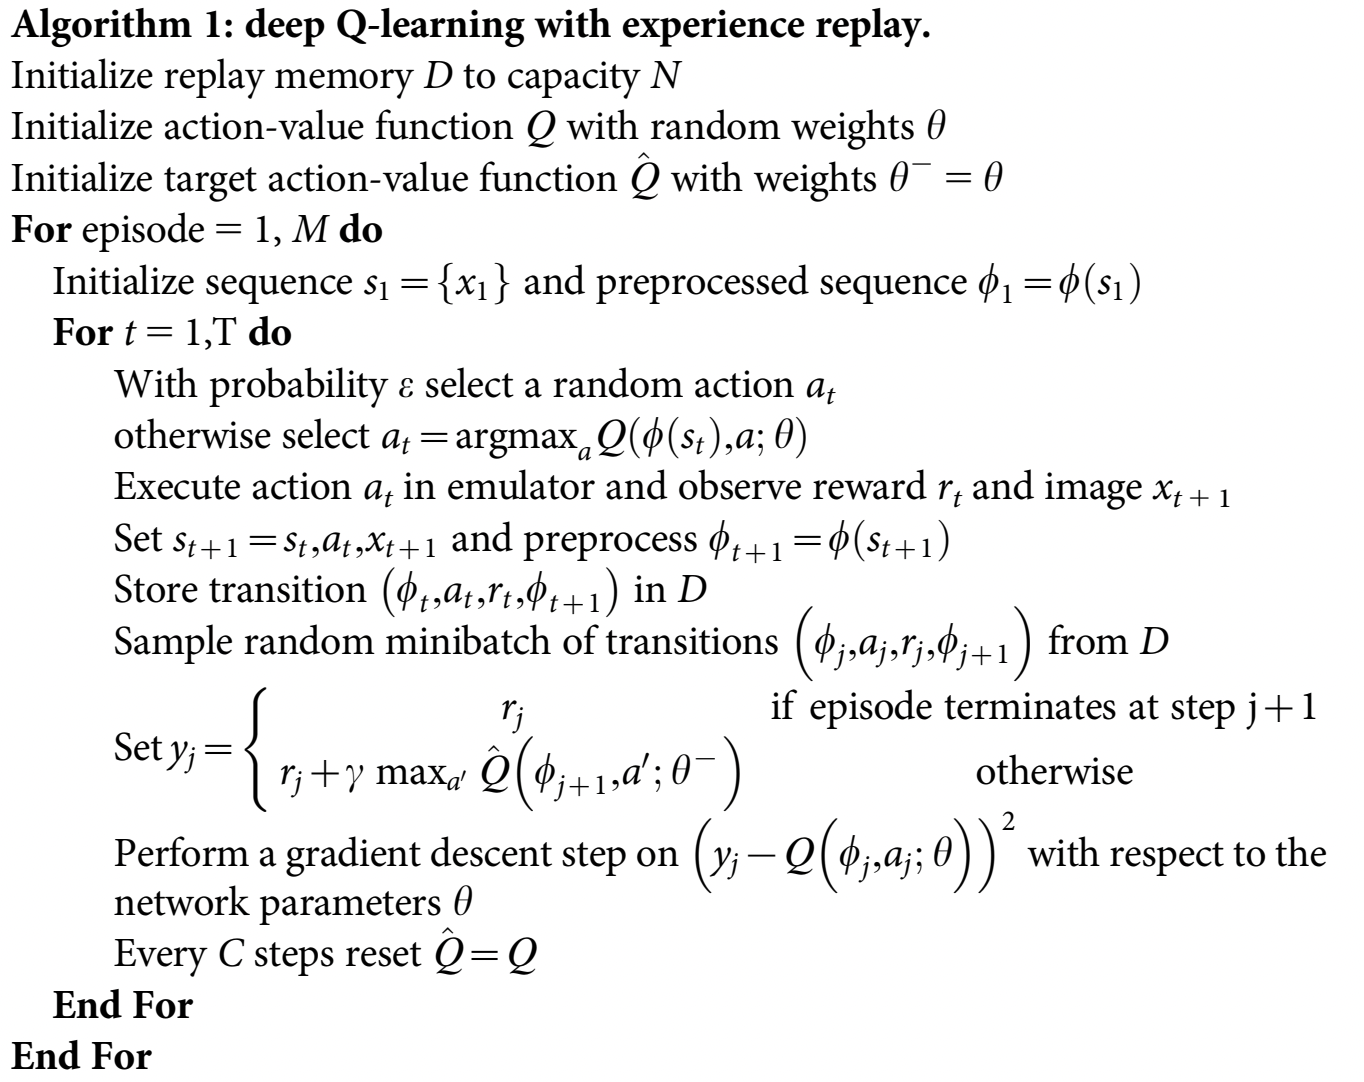
\includegraphics[width=0.8\textwidth]{pictures/dqn_algo_code.png}\\
    \caption[DQN with Experience Replay]{DQN with Experience Replay, as shown in ``Human-level control through deep reinforcement learning'' \cite{mnka15}}\label{fig:dqn_algo_code}
\end{figure}

\marginpar{enhance network}
Executing the selected action results in a memory entry in form of the earlier described quadruple. Afterwards a  minibatch of the replay memory is randomly sampled and used to perform a gradient descent step. The parameter $y_i$ holds information about the target values, if the episode is not about to end. Otherwise, only the reward is assigned to $y_i$. The outcome of the subtraction contains the difference of the target values with the old weights and the current action values with the current network weights.

\marginpar{minibatch advantages}
Finally, every certain amount of steps C the target network is set to the current Q-Network. The suggested process offers several advantages \cite{mnka15}. The replay memory for instance, leads to a smaller deviation or fluctuation in the parameters. The random samples of minibatches can proof to be efficient, since an experience might be used multiple times to update the network weights. Furthermore, through the randomness in the samples the correlation of steps is interrupted, leading to a decrease of variance in between updates. And lastly, updating the target network periodically improves the stability of the learning process.